% !TEX root = main.tex  

\section{Rembering old topics on DNA}

\paragraph{What is DNA made of?}

\begin{itemize}
    \item Pentose sugar (the \emph{sides} of the ladder)
    \item Phosphate group (the \emph{sides} of the ladder)
    \item Nitrogenous bases (the rungs of the ladder)
\end{itemize}

\paragraph{What is a polymer: \\}
Any of a class of natural or synthetic substances composed of very large molecules, called macromolecules.

\paragraph{What is a Nitrogenous base made of?}
\paragraph{\\}
\begin{figure}[htbp]
    \centerline{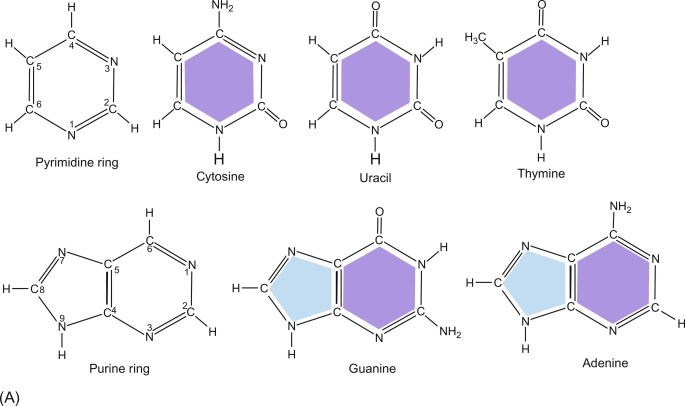
\includegraphics{bases.jpg}}
    \caption{Nitrogenous bases are made of...}
    \label{fig}
\end{figure}

\paragraph{What process can you do with DNA?}

\begin{itemize}
    \item Translation (Protein Synthesis)
    \item Transcription (Synthesizes RNA)
    \item Central Dogma (Transcription + Translation)
\end{itemize}

\paragraph{Where on earth can I find DNA? \\}
The nucleus of a cell contains Chromosomes \\ 
and DNA is contained within the Chromosomes.

\paragraph{\\}
\begin{figure}[htbp]
    \centerline{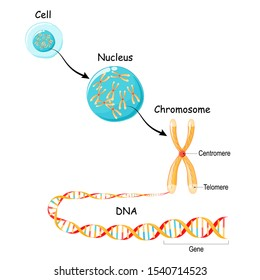
\includegraphics{dna2.jpg}}
    \caption{DNA...}
    \label{fig1}
\end{figure}


\paragraph{Nucleotide composition \\}

\paragraph{\\}
\begin{figure}[htbp]
    \centerline{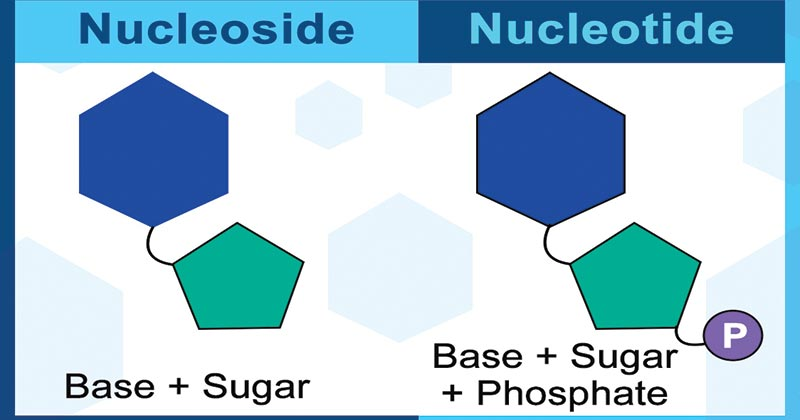
\includegraphics[width=100mm]{nucleotide.jpg}}
    \caption{Here we see a nucleotide and a nucleoside}
    \label{fig2}
\end{figure}

\paragraph{\\}
\paragraph{Remember!}

\begin{itemize}
    \item Humans share 99 of their DNA.
    \item Thymine gets along with Adenine. (hydrogen bonding)
    \item Guanine gets along with Cytosine. (hydrogen bonding)
\end{itemize}

\paragraph{\\}
\begin{figure}[htbp]
    \centerline{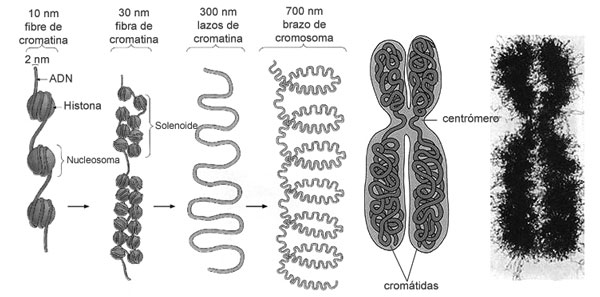
\includegraphics[width=185mm]{adn3.jpg}}
    \caption{A deeper look into Chromosomes}
    \label{fig3}
\end{figure}